\documentclass[12pt]{article}

\usepackage{hyperref}
\usepackage[utf8]{inputenc}
\usepackage{cite}
\usepackage{placeins}
\usepackage{listings}
\usepackage{xcolor}
\usepackage{graphicx}

\linespread{1.5}

\definecolor{listinggray}{gray}{0.9}
\definecolor{lbcolor}{rgb}{0.9,0.9,0.9}

\lstset {
	    backgroundcolor=\color{lbcolor},
	    tabsize=4,    
	    language=[GNU]C++,
        basicstyle=\scriptsize,
        upquote=true,
        aboveskip={1.5\baselineskip},
        columns=fixed,
        showstringspaces=false,
        extendedchars=false,
        breaklines=true,
        prebreak = \raisebox{0ex}[0ex][0ex]{\ensuremath{\hookleftarrow}},
        frame=single,
        numbers=left,
        showtabs=false,
        showspaces=false,
        showstringspaces=false,
        identifierstyle=\ttfamily,
        keywordstyle=\color[rgb]{0,0,1},
        commentstyle=\color[rgb]{0.026,0.112,0.095},
        stringstyle=\color[rgb]{0.627,0.126,0.941},
        numberstyle=\color[rgb]{0.205, 0.142, 0.73}
}

\author{Mikkel Gaub, Malthe Ettrup Kirkbro \& Mads Frederik Madsen}
\title{Thesis Agreement}
\date{\today}

\begin{document}

\maketitle
\thispagestyle{empty}

\vspace{\fill}

\begin{abstract}
Lorem ipsum
\end{abstract}

\pagebreak

\tableofcontents

\pagebreak

	\section{Introduction}

	\section{Related works}

	\section{Background}

		\subsection{Dynamic Condition Response}
		A DCR graph is a representation of a workflow.
		The graph is made up of one or more activities with a number of relations between them. 
		The following section is loosely based on a similar description found in previous work. 

		\subsubsection{Activity}
		The activities in a DCR graph have three attributes: included, executed and pending. 
		The attributes can be true or false. 
		Furthermore an activity can have role and actor specific execution rights.

			\paragraph{Included attribute}
			If the include attribute of an activity is true, the activity is included and it can be executed. 
			If the attribute is false, the activity is excluded and can no longer be executed.

			\paragraph{Pending attribute}
			If any activity in a workflow has a pending attribute that is true and the activity is included, the workflow is in an unfinished state.
			Every time an activity is executed its pending attribute is set to false.
			This means that setting the pending attribute of an included activity to true is specifying that this activity must be executed or excluded at some point to leave the workflow in a finished state.

			\paragraph{Executed attribute}
			If an activities executed attribute is false executing the activity will set its executed attribute to true.
			Executing an already executed activity will have no effect on the executed attribute.

		\begin{figure}[!ht]
			\centering
			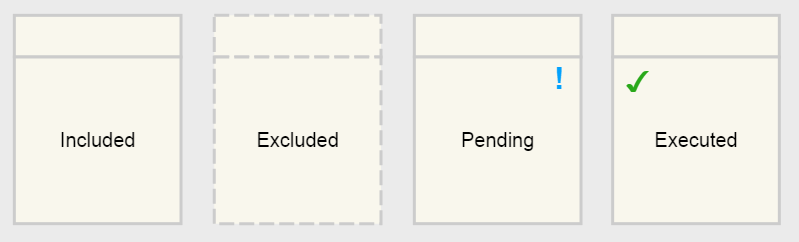
\includegraphics[width=1\textwidth]{figures/activity_states.png}
		 	\caption[Activity States]{From left to right: A visual representation of an included, excluded, pending and executed activity as presented on \href{http://www.dcrgraphs.net}{dcrgraphs.net}}.
		\end{figure}

		\subsubsection{Relations}
		There are five types of relations which define different types of relationships between activities in a workflow. 
		These five are the \emph{condition}, \emph{response}, \emph{include}, \emph{exclude} and \emph{milestone} relations.

			\paragraph{Condition relation}
			If there is a condition relation from activity $A$ to activity $B$, then $B$ can only be executed if $A$'s executed attribute is true or $A$ is excluded.
			\begin{figure}[!ht]
				\centering
				
\includegraphics[width=0.3\textwidth]{figures/ConditionRelation.png}
			 	\caption[Condition relation]
			 	{Condition relation}
			\end{figure}

			\paragraph{Response relation}
			If there is a response relation from activity $A$ to activity $B$, then $B$'s pending attribute will be set to true every time $A$ is executed.
			\begin{figure}[!ht]
				\centering
				
\includegraphics[width=0.3\textwidth]{figures/ResponseRelation.png}
			 	\caption[Response relation]
			 	{Response relation}
			\end{figure}

			\paragraph{Include relation}
			If there is an include relation from activity $A$ to activity $B$, then $B$'s included attribute will be set to true every time $A$ is executed.
			\begin{figure}[!ht]
				\centering
				
\includegraphics[width=0.3\textwidth]{figures/IncludeRelation.png}
			 	\caption[Include relation]
			 	{Include relation}
			\end{figure}

			\paragraph{Exclude relation}
			If there is an exclude relation from activity $A$ to activity $B$, then $B$'s included attribute will be set to false every time $A$ is executed.
			\begin{figure}[!ht]
				\centering
				
\includegraphics[width=0.3\textwidth]{figures/ExcludeRelation.png}
			 	\caption[Exclude relation]
			 	{Exclude relation}
			\end{figure}

			\paragraph{Milestone relation}
			If there is a milestone relation from activity $A$ to activity $B$, then $B$ can only be executed if $A$'s pending attribute is false or $A$'s included attribute is false.
			\begin{figure}[!ht]
				\centering
				
\includegraphics[width=0.3\textwidth]{figures/MilestoneRelation.png}
			 	\caption[Milestone relation]
			 	{Milestone relation}
			\end{figure}

		\subsection{SGX}

		\subsection{Consensus}

	\section{Challenges}

		\subsection{SGX}

		\subsection{Consensus}	

	\section{Implementation}

	\section{Conclusion}

	\begin{thebibliography}{9}

		\bibitem{dcreum}
		Mikkel Gaub, Tróndur Høgnason, Malthe Ettrup Kirkbro \& Mads Frederik Madsen.
		\textit{Consensus in declarative process models using distributed smart-contracts}.

	\end{thebibliography}

\end{document}